% Created 2017-10-26 Thu 19:07
\documentclass[presentation]{beamer}
\usepackage[utf8]{inputenc}
\usepackage[T1]{fontenc}
\usepackage{fixltx2e}
\usepackage{graphicx}
\usepackage{longtable}
\usepackage{float}
\usepackage{wrapfig}
\usepackage{rotating}
\usepackage[normalem]{ulem}
\usepackage{amsmath}
\usepackage{textcomp}
\usepackage{marvosym}
\usepackage{wasysym}
\usepackage{amssymb}
\usepackage{hyperref}
\tolerance=1000
\usepackage{tabu}
\usepackage{minted}
\usepackage[english, ngerman]{babel}
\hypersetup{pdfauthor="Vasilij Schneidermann", pdftitle="Klavier spielen mit Kawa Scheme", colorlinks, linkcolor=black, urlcolor=blue}
\uselanguage{German}
\languagepath{German}
\usetheme{Rochester}
\usecolortheme[RGB={87,83,170}]{structure}
\author{Vasilij Schneidermann}
\date{Oktober 2017}
\title{Klavier spielen mit Kawa Scheme}
\hypersetup{
  pdfkeywords={},
  pdfsubject={},
  pdfcreator={Emacs 25.3.1 (Org mode 8.2.10)}}
\begin{document}

\maketitle
\begin{frame}{Outline}
\tableofcontents
\end{frame}

\AtBeginSection{\frame{\sectionpage}}
\shorthandoff{"}

\section{Intro}
\label{sec-1}

\begin{frame}[label=sec-1-1]{Sprecher}
\begin{itemize}
\item Vasilij Schneidermann, 25
\item Software-Entwickler bei \href{https://www.bevuta.com/en/}{bevuta IT GmbH}
\item mail@vasilij.de
\item \url{https://github.com/wasamasa}
\item \url{http://emacshorrors.com/}
\item \url{http://emacsninja.com/}
\end{itemize}
\end{frame}

\begin{frame}[label=sec-1-2]{Motivation}
\begin{itemize}
\item Keine Musikausbildung
\item Ich möchte gerne Musik covern, vielleicht komponieren
\item MIDI-Keyboards sind sperrig
\item DAWs zu fokussiert auf Synthesizer
\item GUI Kompositions-Software lenkt ab
\item Tracker: glorifizierter Hexeditor
\item Idee: Workflow wie im Texteditor
\item Nutzung von MIDI, ggf. OSC
\end{itemize}
\end{frame}

\begin{frame}[label=sec-1-3]{Screenshots (Reason 8)}
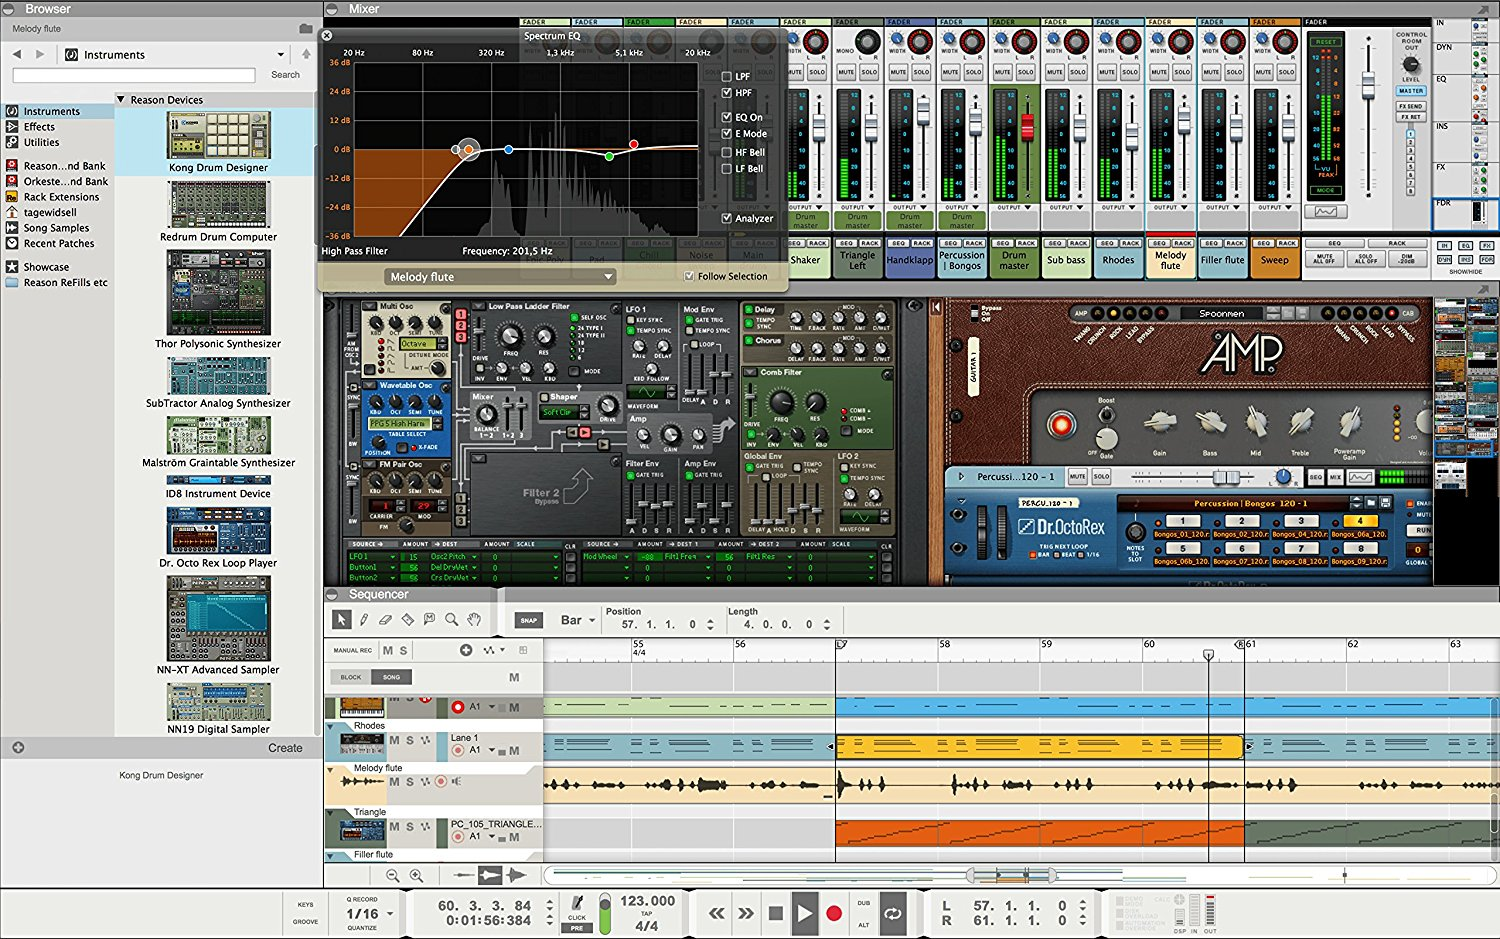
\includegraphics[width=.9\linewidth]{./scrots/reason8.jpg}
\end{frame}

\begin{frame}[label=sec-1-4]{Screenshots (Sibelius 7)}
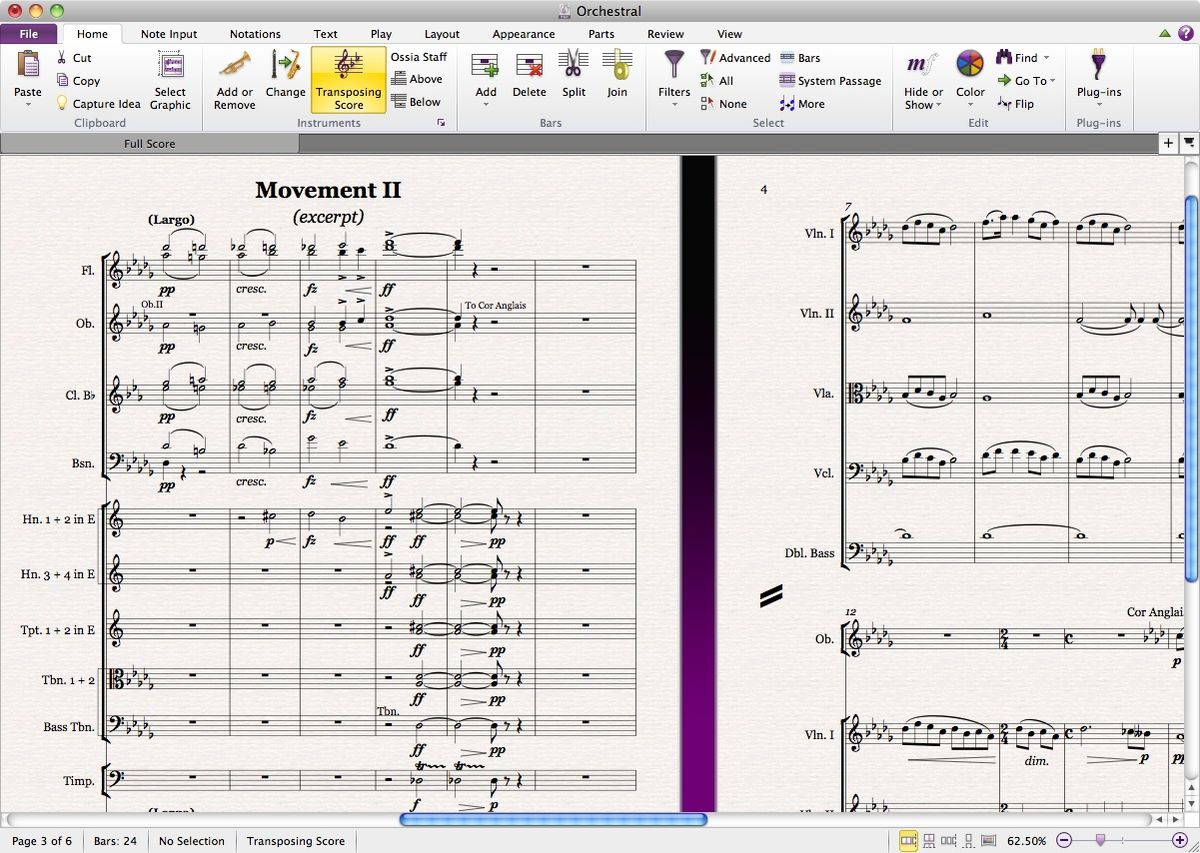
\includegraphics[width=.9\linewidth]{./scrots/sibelius7.jpg}
\end{frame}

\begin{frame}[label=sec-1-5]{Screenshots (Milkytracker)}
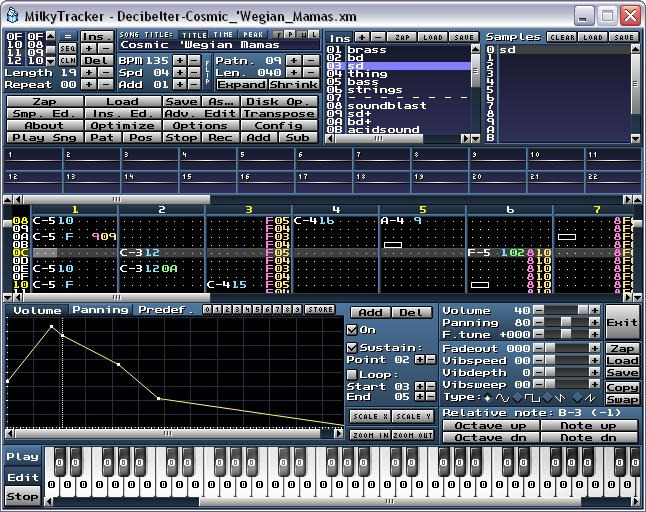
\includegraphics[width=.9\linewidth]{./scrots/milkytracker.jpg}
\end{frame}

\begin{frame}[label=sec-1-6]{Inspiration für dieses Projekt}
\begin{itemize}
\item \url{https://blog.djy.io/alda-a-manifesto-and-gentle-introduction/}
\item Ziemlich genau was ich suche
\item Aber: Clojure ist suboptimal dafür
\item Zu komplex (Größe der Codebase, Dependencies, Architektur)
\item Fehlendes Feature: Free Play
\item Funktioniert nicht richtig (manuelles Netzwerksetup nötig)
\item Kriege ich das besser hin?
\end{itemize}
\end{frame}

\begin{frame}[label=sec-1-7]{JVM-Sprachen}
\begin{itemize}
\item Clojure (modernes Lisp-1)
\item Scala (OOP, funktional, Sammelsurium an Features)
\item JRuby / Jython (Ruby / Python)
\item Groovy (nicht weiter besonders)
\item Kotlin (neu, von Jetbrains)
\item Frege (Haskell)
\item Kawa / JScheme / SISC (Scheme)
\end{itemize}
\end{frame}

\begin{frame}[fragile,label=sec-1-8]{Kawa}
 \begin{itemize}
\item Existiert seit 1998, unterstützt die gängigen Standards (R5RS, R6RS,
R7RS)
\item Implementiert viele SRFIs und hat eigene Erweiterungen
\item Start: 1s, Kompilieren: 1s, Geschwindigkeit: akzeptabel
\item Interop mit Java funktioniert gut, inklusive Generieren von Klassen
\item Hohe Qualität, bisher nur Dokumentationsbugs gefunden
\item Hauptnachteil: Kaum eigenes Tooling (Dokumentation verweist auf
\texttt{ant}\ldots{})
\end{itemize}
\end{frame}

\begin{frame}[fragile,label=sec-1-9]{Waka}
 \begin{itemize}
\item Sorry für den Namen
\item Dependencies: JLine3 (Terminal-Support), \texttt{javax.sound.midi}
  (Generieren, verarbeiten und abspielen von MIDI)
\item Live Demo!
\end{itemize}
\end{frame}

\section{Grundlagen}
\label{sec-2}

\begin{frame}[label=sec-2-1]{MIDI}
\begin{itemize}
\item Universeller Standard zum Übertragen von Musik-Events
\item Transmitters / Receivers
\item MIDI-Controller (Keyboards)
\item MIDI-Sequencer
\item MIDI-Synthesizer
\item MIDI-Kabel
\item Dateityp: Standard MIDI File
\item Soundbanks, Soundfont-Format
\end{itemize}
\end{frame}

\begin{frame}[label=sec-2-2]{MIDI-Limitierungen}
\begin{itemize}
\item 16 Channels (jeder pro Gerät/Synthesizer)
\item Channel 9 ist für Perkussion
\item Tracks für logische Gruppierung
\item Dateien können aus einem (Type 0) oder mehreren (Type 1) Tracks
oder mehreren Songs (Type 2) bestehen
\item 128 Instrumente in 16 Gruppen (General MIDI Standard)
\item Besondere Events für Lautstärke, Pitch Bending, Tempo, \ldots{}
\item Längen werden in Ticks gemessen, Länge eines Ticks ist an den
gesamten Song gebunden
\end{itemize}
\end{frame}

\begin{frame}[fragile,label=sec-2-3]{\texttt{javax.sound.midi}}
 \begin{itemize}
\item Java SE hat \texttt{javax.sound.sampled} (Low-level Audiowiedergabe) und
\texttt{javax.sound.midi} (vollständige MIDI-Implementierung)
\item Features:
\begin{itemize}
\item MIDI parsen
\item Soundbanks laden
\item Einzelne Noten spielen
\item Sequences generieren
\item Sequences mit einem Sequencer spielen
\item Sequences speichern
\item Viele Klassen die MIDI weitestgehend abdecken
\end{itemize}
\end{itemize}
\end{frame}

\begin{frame}[fragile,label=sec-2-4]{JLine3}
 \begin{itemize}
\item Optionale Dependency für Kawa
\item Free Play erfordert sofortige Reaktion auf gedrückte Taste
\item Möglich durch Aktivieren eines \emph{raw mode} (Deaktivieren nicht
vergessen!)
\item Ermöglicht \texttt{SIGINT} abzufangen damit die JVM nicht abstürzt
\item Bonus-Features: Line editing, persistente History
\end{itemize}
\end{frame}

\section{MIDI-Beispiele (Code)}
\label{sec-3}

\begin{frame}[fragile,label=sec-3-1]{Init}
 \begin{minted}[]{scheme}
(set! synthesizer (MidiSystem:getSynthesizer))
(Synthesizer:open synthesizer)
(set! sequencer (MidiSystem:getSequencer))
(Sequencer:open sequencer)
(let ((transmitter (Sequencer:getTransmitter sequencer))
      (receiver (Synthesizer:getReceiver synthesizer)))
  (transmitter:setReceiver receiver))

(set! channels (Synthesizer:getChannels synthesizer))
(set! channel (channels channel-id))
\end{minted}
\end{frame}

\begin{frame}[fragile,label=sec-3-2]{Init}
 \begin{minted}[]{scheme}
(set! soundbank
      (if soundbank-path
          (MidiSystem:getSoundbank (File soundbank-path))
          (Synthesizer:getDefaultSoundbank synthesizer)))

(set! instruments (Soundbank:getInstruments soundbank))
(set! instrument-id (or instrument-id 0))
(set! instrument
      (if (< instrument-id instruments:length)
          (instruments instrument-id)
          (instruments 0)))

(Synthesizer:loadInstrument synthesizer instrument)
(MidiChannel:programChange channel instrument-id)
\end{minted}
\end{frame}

\begin{frame}[fragile,label=sec-3-3]{Noten spielen}
 \begin{minted}[]{scheme}
;; traditional way
(MidiChannel:noteOn channel midi-note velocity)
(MidiChannel:noteOff channel midi-note velocity)

;; alternative way
(MidiChannel:noteOn channel midi-note velocity)
(MidiChannel:noteOn channel midi-note 0)
\end{minted}
\end{frame}

\begin{frame}[fragile,label=sec-3-4]{Sequence generieren}
 \begin{minted}[]{scheme}
(define (add-note-on track start key velocity)
  (let ((note (ShortMessage)))
    (note:setMessage ShortMessage:NOTE_ON
                     channel-id key velocity)
    (Track:add track (MidiEvent note start))))

(define (add-silent-note track start key)
  (add-note-on track start key 0))

(define (add-note track start length key velocity)
  (add-note-on track start key velocity)
  (add-silent-note track (+ start length) key))
\end{minted}
\end{frame}

\begin{frame}[fragile,label=sec-3-5]{Sequence generieren}
 \begin{minted}[]{scheme}
(let* ((sequence (Sequence Sequence:PPQ 32))
       (track (sequence:createTrack))
       ;; C D E F G A B
       (notes '(60 62 64 65 67 69 71)))
  (let loop ((notes notes)
             (start 0))
    (when (pair? notes)
      (add-note-on track start 30 note 127)
      (loop (cdr notes) (+ start 32)))))
\end{minted}
\end{frame}

\begin{frame}[fragile,label=sec-3-6]{Sequence abspielen}
 \begin{minted}[]{scheme}
(Sequencer:setSequence sequencer midi)
(Sequencer:setTempoInBPM sequencer bpm)
(Sequencer:start sequencer)
\end{minted}
\end{frame}

\begin{frame}[fragile,label=sec-3-7]{Sequence speichern}
 \begin{minted}[]{scheme}
(let ((midi (sequence->midi sequence))
      (version (if (multi-track-sequence? sequence)
                   1
                   0)))
  (MidiSystem:write midi version (File out-path)))
\end{minted}
\end{frame}

\section{Tour durch waka}
\label{sec-4}

\begin{frame}[label=sec-4-1]{Features}
\begin{itemize}
\item Free Play (jedes getippte Zeichen lässt eine Note erklingen)
\item REPL-Mode (synthetisieren einer Zeile Code) mit History
\item Parsen eines Subsets von Alda-Syntax
\item Einfache Fehlerbehandlung mit Fehlermeldungen à la GCC
\item Konfigurationsdatei
\item Batch-Mode für MIDI- und waka-Dateien
\item Konvertieren von waka- zu MIDI-Dateien
\item Implementiert in <1000 SLOC (Alda umfasst 7000 SLOC)
\end{itemize}
\end{frame}

\begin{frame}[fragile,label=sec-4-2]{Free Play}
 \begin{itemize}
\item Wie ein billiges MIDI-Keyboard
\item Konvertiert gedrückte Taste zu Note und erzeugt ein \texttt{NoteOn}-Event
\item Zeigt die Note mit der korrekten Syntax an (praktisch für Copy-Paste)
\item Eigene Keymap möglich
\item Oktavenwechsel mit \texttt{<} und \texttt{>}
\item Wechseln zum REPL-Mode mit \texttt{C-SPC}
\item Workflow: Ausprobieren von Noten, Komponieren in REPL-Mode
\end{itemize}
\end{frame}

\begin{frame}[fragile,label=sec-4-3]{REPL-Mode}
 \begin{itemize}
\item Parsen einer einfachen Notensyntax zu einem AST
\item \texttt{RET} synthetisiert eine MIDI-Sequence und spielt sie ab
\item Line Editing dank JLine3
\item Workflow: Editieren und Abspielen der aktuellen Zeile bis es richtig
klingt, fertige Zeilen werden in eine waka-Datei kopiert
\end{itemize}
\end{frame}

\begin{frame}[label=sec-4-4]{Batch-Mode}
\begin{itemize}
\item Parsen mehrerer Tracks zu einer Liste von ASTs
\item Konvertieren dieser zu einer mehrspurigen MIDI-Sequence
\item Abspielen oder Speichern der Sequence
\item Verbesserungsmöglichkeit: Ausgabe des ASTs für Export zu beliebigen
Formaten
\end{itemize}
\end{frame}

\begin{frame}[fragile,label=sec-4-5]{Syntax}
 \begin{itemize}
\item Noten: \texttt{c d e f g a b}
\item Notenwert: \texttt{c1 c2 c4 c8 c16 c32}
\item Punktierte Note (verlängert den Wert um 1.5): \texttt{c d e.}
\item Haltebogen: \texttt{c1\textasciitilde{}1}
\item Notenwert ist anfangs $1\over{4}$ und wird bis zum nächsten
angegebenem Wert beibehalten: \texttt{c4 d e f g2 g}
\item Versetzungszeichen: \texttt{c c+ c- c\_}
\end{itemize}
\end{frame}

\begin{frame}[fragile,label=sec-4-6]{Syntax}
 \begin{itemize}
\item Akkorde: \texttt{c/e/g c/e-/g}
\item Pausen: \texttt{r4 r1\textasciitilde{}1 r}
\item Taktstriche (werden ignoriert): \texttt{r1 r r r | r2 r | r4}
\item Oktave versetzen: \texttt{a > c e r2 e c < a}
\item Oktave wechseln: \texttt{o0 c o2 c o4 c o6 c o8 c}
\item S-Expressions: \texttt{(tempo 120) (tempo)}
\item Kommentare: \texttt{\# you won't see me}
\end{itemize}
\end{frame}

\begin{frame}[fragile,label=sec-4-7]{Sequences vs Scores}
 \begin{itemize}
\item Sequence besteht aus durch Leerzeichen getrennten Worten
\item \texttt{c4 d e f | g2 g}
\item Score besteht aus Sequences, jede wird mit einem Namen eingeleitet
\item \texttt{main: o4 c1 d e f g a b > c}
\item \texttt{backing: o4 c1 < b a g f e d < c}
\end{itemize}
\end{frame}

\begin{frame}[fragile,label=sec-4-8]{Lexing}
 \begin{itemize}
\item Im ersten Schritt werden Kommentare entfernt, Wörter anhand von
Leerzeichen aufgeteilt, Tokens und S-Expressions eingelesen
\item Ein String-Port hält den aktuelle State fest
\item Die gefundenen Tokens / S-Expressions werden in einer Liste
gesammelt
\item Das Prinzip des String-Ports kann auf Tokens übertragen werden,
dafür werden die Funktionen \texttt{peek-token} / \texttt{read-token} definiert
\end{itemize}
\end{frame}

\begin{frame}[fragile,label=sec-4-9]{Ports (Code)}
 \begin{minted}[]{scheme}
(define port (open-input-string "abc"))
(peek-char port) ;=> a
(read-char port) ;=> a
(peek-char port) ;=> b
(read-char port) ;=> b
(read-char port) ;=> c
(read-char port) ;=> #!eof
\end{minted}
\end{frame}

\begin{frame}[fragile,label=sec-4-10]{Lexing (Code)}
 \begin{minted}[]{scheme}
(let loop ((tokens '()))
  (let ((char (peek-char port)))
    (if (eof-object? char)
        (reverse tokens)
        (cond ((whitespace? char)
               (read-whitespace port) (loop tokens))
              ((eqv? char #\#)
               (read-line port) (loop tokens))
              ((eqv? char #\()
               (loop (cons (read port) tokens)))
              (else
               (loop (cons (read-token port) tokens)))))))
\end{minted}
\end{frame}

\begin{frame}[fragile,label=sec-4-11]{Lexing (Code)}
 \begin{minted}[]{scheme}
(define (whitespace? char)
  (or (char-whitespace? char) (eqv? char #\|)))
(define (read-whitespace port)
  (let loop ()
    (when (whitespace? (peek-char port))
      (read-char port))))
(define (read-token port)
  (let loop ((chars '()))
    (let ((char (peek-char port)))
      (if (and (not (eof-object? char))
               (not (whitespace? char))
               (not (memv char '(#\; #\())))
          (loop (cons (read-char port) chars))
          (list->string (reverse chars))))))
\end{minted}
\end{frame}

\begin{frame}[fragile,label=sec-4-12]{Parsing}
 \begin{itemize}
\item Handgeschriebener Recursive Descent Parser
\item Die Sprache wird durch eine Grammatik in EBNF beschrieben
\item Jede Regel der Grammatik wird zu einer Funktion übersetzt die einen
Token-Port oder String-Port akzeptiert und Teil des AST zurückgibt
\item Wenn eine Regel nicht genutzt werden kann, wird \texttt{\#f} zurückgegeben
\item Fehler brechen das Parsen ab und werden in der REPL angezeigt
\item Macht den meisten Code aus (> 200 SLOC)
\end{itemize}
\end{frame}

\begin{frame}[fragile,label=sec-4-13]{Parsing (Grammar \& Code)}
 \begin{minted}[]{scheme}
;; note = key { modifier } .

(define (read-note port)
  (let ((key (read-key port)))
    (if key
        (let loop ((modifiers '()))
          (let ((modifier (read-modifier port)))
            (if modifier
                (loop (cons modifier modifiers))
                `(note (key . ,key)
                       ,@(reverse modifiers)))))
        #f)))
\end{minted}
\end{frame}

\begin{frame}[fragile,label=sec-4-14]{Parsing (Grammar \& Code)}
 \begin{minted}[]{scheme}
;; key = "a" | "b" | "c" | "d" | "e" | "f" | "g" .

(define (read-key port)
  (if (memv (peek-char port)
            '(#\a #\b #\c #\d #\e #\f #\g))
      (read-char port)
      #f))
\end{minted}
\end{frame}

\begin{frame}[fragile,label=sec-4-15]{Fehlerbehandlung}
 \begin{verbatim}
midi> cxxx
Error: Trailing garbage
cxxx
 ^^^
\end{verbatim}

\begin{itemize}
\item Fehlerbehandlung und Parsen sind verwoben
\item Bei Fehlern in einem Token wird die aktuelle Spalte vom String-Port
extrahiert und auf diese Spalte im Token gezeigt
\item Der letzte Token wird in einem Parameter-Object festgehalten
\item Alle anderen Fehler werfen eine einfache Fehlermeldung
\end{itemize}
\end{frame}

\begin{frame}[fragile,label=sec-4-16]{Fehlerbehandlung (Code)}
 \begin{minted}[]{scheme}
(guard
 (ex
  ((parse-error-object? ex)
   (display "Error: ")
   (print (parse-error-message ex))
   (let* ((token (parse-error-token ex))
          (indent (port-column (parse-error-port ex)))
          (width (string-length token)))
     (print token)
     (display (make-string indent #\space))
     (display (make-string (max (- width indent) 1) #\^))
     (newline)
     (loop)))
  ...)
 ...)
\end{minted}
\end{frame}

\begin{frame}[fragile,label=sec-4-17]{Bonus: Promises mit asynchronen APIs}
 \begin{itemize}
\item Problem: \texttt{javax.sound.midi} ist teilweise asynchron
\item Abspielen einer MIDI-Sequence blockiert nicht, Interpreter wird
sofort beendet
\item Lösung: Blockierende API erzeugen mit einem Promise
\item Promise hört auf zu blockieren sobald ein Wert gesetzt wurde
\item Promise wird in einem Event Handler aufgelöst wenn es ein EOT-Event
ist
\end{itemize}
\end{frame}

\begin{frame}[fragile,label=sec-4-18]{Bonus: Promises mit asynchronen APIs (Code)}
 \begin{minted}[]{scheme}
(let ((done (promise)))
  (sequence-thunk)
  (Sequencer:addMetaEventListener
   sequencer
   (lambda (message)
     (when (= (MetaMessage:getType message) END-OF-TRACK)
       (promise-set-value! done #t)
       (quit!))))
  (Sequencer:start sequencer)
  (force done))
\end{minted}
\end{frame}

\begin{frame}[fragile,label=sec-4-19]{Bonus: Uberjar}
 \begin{itemize}
\item Problem: Es ist etwas nervig sich Kawa mit JLine3 einzurichten
\item Lösung: Konstruktion einer JAR-Datei die alle nötigen class-Dateien
beinhaltet um waka auszuführen
\item Problem: Es gibt keine fertigen allgemeintauglichen Tools dafür,
empfohlen werden \texttt{ant}, \texttt{maven} und Enterprise-taugliche Projekte
mit eigenem Class Loader
\item Lösung: Händisches Erstellen eines Uberjars und Automatisierung mit
GNU Make
\item \url{https://github.com/wasamasa/waka/blob/master/Makefile}
\end{itemize}
\end{frame}

\begin{frame}[fragile,label=sec-4-20]{Bonus: Grafisches Debugging}
 \begin{itemize}
\item Problem: Debugging mit dem Ohr ist schwierig
\item Lösung: Konvertierung und Export zu Lilypond
\item Lilypond beinhaltet einen Batch-Mode für die Konvertierung von
Lilypond-Dateien zu PDF
\item Lilypond hat ein \texttt{midi2ly}-Skript
\item \texttt{waka2ly} ist ein stupides Shell-Skript das von waka nach MIDI nach
Lilypond konvertiert
\end{itemize}
\end{frame}

\section{Outro}
\label{sec-5}

\begin{frame}[label=sec-5-1]{Fehlende Features}
\begin{itemize}
\item Auto-Completion für S-Expressions in REPL-Mode
\item Support für Channels, mehrere Instrumente, Instrument-Aliase
\item Perkussion (Channel 9)
\item Vorzeichen für eine Sequence, Auflösungszeichen
\item Legato / Pedal
\item Syntax für Wiederholung von Noten und Gruppen
\item Beliebige Längen für Noten und Sequences (Triolen / CRAM)
\item Arpeggio, Glissando / Portamento, andere Artikulation
\end{itemize}
\end{frame}

\begin{frame}[label=sec-5-2]{Weitere Pläne}
\begin{itemize}
\item Qualität an Alda angleichen, nützliche Features erkennen und
\sout{klauen} übernehmen
\item Mehr Notenblätter \sout{abschreiben} übersetzen
\item Mechanismus für einen allgemeinen Import / Export (z.B. MIDI Import,
Lilypond Export)
\item Debug-Modus, Testbarkeit ermöglichen (Analyse von generiertem MIDI)
\item Verbessern der vorhandenen Tests
\end{itemize}
\end{frame}

\begin{frame}[label=sec-5-3]{Mehr Musik}
\begin{itemize}
\item Popcorn
\end{itemize}
\end{frame}

\begin{frame}[label=sec-5-4]{Fragen?}
\end{frame}
% Emacs 25.3.1 (Org mode 8.2.10)
\end{document}